\documentclass{standalone}
\begin{document}

\chapter*{Introduction}\addcontentsline{toc}{chapter}{Introduction}
\markboth{Itroduction}{Introduction}


Since the end of 2019, COVID-19 has widely spread all over the world. Up to now the gold standard for the identification of the pathology is the RT-PCR even if it is reported that its sensitivity might not be enough for COVID-19 identifications~\cite{ART:Ai} and requires a lot of time to provide results.\\
Up to now the gold standard for the diagnosis of this disease are the reverse transcription-polymerase chain reaction (RT-PCR) and the gene sequencing of sputum, throat swab and lower respiratory tract secretion~\cite{ART:Zhao}.\\ Many COVID-19 affected patients have shown ground glass opacities(GGO) and consolidation(CS) in chest CT, which are also made in relation with the stage of the disease ~\cite{ART:Bernheim}.  As shown by \cite{ART:Huang}, initial prospective analysis have shown that the $98\%$ have bilateral patchy shadows or ground glass opacity (GGO) and consolidation(CS) in lung. Other study have have monitored the change on volume and shape of these features on healed patients~\cite{ART:Ai} in order to monitoring their recovery. In \figurename\,\ref{fig:HealthVSCovid} are compared slices of an healthy control and a patient affected by COVID-19. We can clearly see the GGO and CS regions in the lung of the second one.\\
	
\begin{figure}[h!]
	\centering
	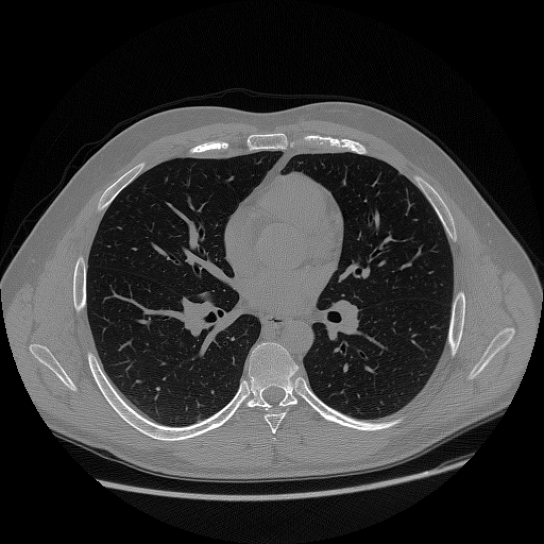
\includegraphics[scale=.5]{healthy.png}
	\quad
	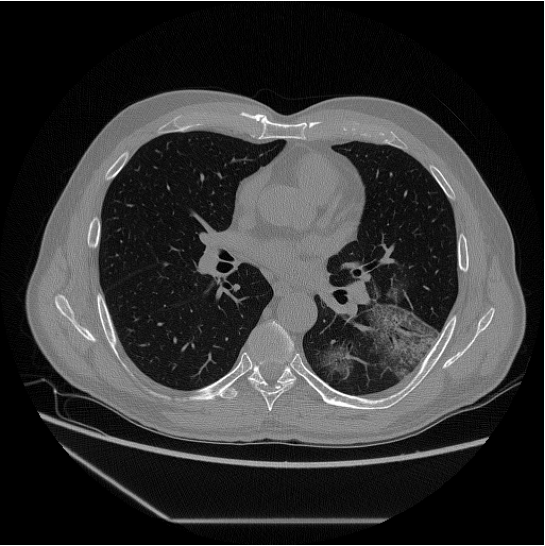
\includegraphics[scale=.5]{ggo.png}
	\label{fig:HealthVSCovid}\caption{CT scan of thorax for an healthy patient(left) and a COVID-19 affected one(right) in which we can observe a huge amount of GGO in the right lung}
\end{figure} 


GGO and CS are not exclusive of COVID-19, but may be also caused by pulmonary edema, bacterial infection, other viral infection or alveolar haemorrage~\cite{ART:Collins}. However the combination between CT scan information and other diagnostic tehcniques like the RT-PCR mentioned above, may help the diagnosis, the monitoring of the course of the disease and the checking of the recovery in healed patients. Since COVID-19 is a new disease, the study of these features in COVID-19 affected patients may help the understanding of the infection pathogenesis.\\
Austin in Glossary of terms for CT of the lungs~\cite{ART:Austin} define the Ground Glass Opacities as \emph{hazy increased attenuation of lung, with preservation of bronchial and vascular margins caused by partial filling of air spaces, interstitial thickening, partial collapse of alveoli, normal expiration, or increased capillary blood volume}.
For the reason given before, the identification of this kind of lesions in CT scans of lung is very important. Up to now the segmentation is made in a manual or semiautomatic way, which are time consuming and subjective, since involves the interaction with trained personnel. AN automatic and fast way for the identification of this features is desired.\\
In this thesis work I will present an automatic and fast pipeline for the identification of these kind of lesions. The pipeline was developed by using $83$ chest CT scans of COVID-19 affected patients, kindly provided by Sant'Orsola hospital. Also scans from two public dataset (ZENODO~\cite{DATA:ZENODO}, MOSMED~\cite{DATA:MOSMED}) where used as benchmark.\\
The developed pipeline is completely unsupervised and its based on the cclor quantization, so the relation between the HU and the different linear attenuation coefficient of tissues is exploited. In order to takes into account other features, like the spatial extension of the lesion areas, or the different shape of the lung structure, a suitable color space was build.\\
The pipeline was implemented in python and to perform the different operations different image processing libraries where used : \emph{SimpleITK}, \emph{OpenCV} and \emph{scikit-image}.\\
The time performance of the pipeline are verified on the DIFA servers and the segmentation accuracy on labels provided by the manual segmentation performed by and expert.

\end{document}